% Build: make paper (latexmk -pdf main.tex). Tables *.gen.tex and plots/*.gen.tex
% are generated by cmd/eval-* and cmd/plots from output/; do not edit them.
\documentclass[11pt]{article}
\usepackage[margin=2.5cm]{geometry}
\usepackage{booktabs,amsmath,amssymb,graphicx,url,hyperref,pgfplots}
\pgfplotsset{compat=1.18}
\usepackage[numbers]{natbib}

\title{Many Options, One Call: Diagnosing and Repairing System~1 Decision Models\\at Large Option Counts with Tournament Querying and a Conformal Survival Guarantee}
\author{Miko\l{}aj Semeniuk}
\date{\today}

\begin{document}
\maketitle

\begin{abstract}
% TODO: 150-200 words. Problem: one /v1/systemone call with k options degrades
% in accuracy, order sensitivity and calibration as k grows (Laya collapses
% between k=24 and k=59 because of its 192-token option budget; Kev degrades
% smoothly). Method: tournament querying (groups of G, winners to a final),
% adaptive threshold eps, conformal selection of eps with a survival guarantee.
% Results: Laya CLINC150 k=150 0.53 -> 0.84 with 8 calls / 219 ms, above Kev-9B
% single call (0.79, 1.1 s) and Qwen2.5-7B (0.79, 0.9 s); tournament hurts Kev
% (per-round errors compound) and permutation averaging is the right tool
% there; 44/45 certified eps hold on test. Release: Go harness + data.
\end{abstract}

\section{Introduction}
% TODO
% - System 1 decision models (Laya, Kev, Jev, Decision-1): one forward pass,
%   probabilities over named options, served by llama.cpp /v1/systemone.
% - Real tasks have many options: 77 banking intents, 150 CLINC intents,
%   255 tools (API cap). Prior work measured the drop and said "keep k <= 10"
%   \citep{fastmodels2026}; nobody tested a repair.
% - Contributions: (1) diagnosis across 4 models x 6 datasets x k in 3..255,
%   (2) tournament / adaptive / chain querying, (3) conformal eps selection
%   with a certified survival bound, (4) finding: helps encoders with a
%   token budget, hurts decoder-based pointer models; rule of thumb
%   accuracy(tournament) ~ product of per-round accuracies.

\section{Related work}
% TODO: System 1 decision models \citep{fastmodels2026,rafedas2026,jevout2026,
% typesafe2026,system1arena2026,llmasjev2026,pentest2026}; cascades
% \citep{cab2025}; order sensitivity of LLM multiple choice
% \citep{lu2022order,zheng2023mcq}; calibration \citep{guo2017calibration};
% conformal risk control \citep{angelopoulos2022crc,angelopoulos2021ltt,
% angelopoulos2021gentle}.

\section{Setup}
\subsection{Models and serving}
% TODO: Laya (ModernBERT-large 421M, [MASK] scoring, 192-token option budget,
% max 255 options), Kev-0.8B/4B/9B (Qwen3.5 + LoRA + pointer head), BF16 GGUF
% on llama.cpp b11559 \citep{llamacpp}, one llama-server per model, ASUS Ascent
% GX10 (GB10, 128 GB). LLM reference: Qwen2.5-7B-Instruct Q4\_K\_M \citep{qwen25}.
\subsection{Datasets}
% TODO: Emotion (6), XNLI (3), MASSIVE (59), Banking77 (77), CLINC150 (150)
% \citep{larson2019clinc}, BFCL function selection (453 functions, descriptions)
% \citep{bfcl2024}. 50/50 calibration/test split, seed 0. Distractor sampling:
% gold + k-1 random options, fixed per (example, k).
\subsection{Metrics}
% TODO: accuracy, macro-F1, ECE (10 bins), Brier, flip rate (sorted vs
% reversed), survival (gold among finalists), calls per decision, p50/p95
% latency (one worker, one model at a time for the cost tables).

\section{Diagnosis: one call with $k$ options}
% generated by cmd/eval-baseline, do not edit
\begin{tabular}{llrrrrrr}
\toprule
Dataset & Model & $k$ & Acc & F1 & ECE & Brier & p50 (ms) \\
\midrule
banking77 & kev-0.8b & 77 & 0.824 & 0.819 & 0.145 & 0.289 & 89.1 \\
banking77 & kev-4b & 77 & 0.856 & 0.853 & 0.132 & 0.239 & 304.5 \\
banking77 & kev-9b & 77 & 0.858 & 0.856 & 0.025 & 0.213 & 529.5 \\
banking77 & laya & 77 & 0.365 & 0.322 & 0.612 & 1.237 & 28.4 \\
clinc150 & kev-0.8b & 150 & 0.656 & 0.654 & 0.200 & 0.525 & 232.0 \\
clinc150 & kev-4b & 150 & 0.800 & 0.806 & 0.314 & 0.404 & 737.7 \\
clinc150 & kev-9b & 150 & 0.813 & 0.807 & 0.190 & 0.316 & 1123.2 \\
clinc150 & laya & 150 & 0.491 & 0.469 & 0.481 & 0.977 & 83.5 \\
emotion & kev-0.8b & 6 & 0.560 & 0.457 & 0.053 & 0.587 & 64.7 \\
emotion & kev-4b & 6 & 0.564 & 0.476 & 0.067 & 0.593 & 231.9 \\
emotion & kev-9b & 6 & 0.567 & 0.468 & 0.060 & 0.593 & 397.6 \\
emotion & laya & 6 & 0.603 & 0.505 & 0.289 & 0.676 & 15.0 \\
massive & kev-0.8b & 59 & 0.642 & 0.630 & 0.153 & 0.517 & 62.1 \\
massive & kev-4b & 59 & 0.719 & 0.697 & 0.235 & 0.451 & 236.3 \\
massive & kev-9b & 59 & 0.729 & 0.718 & 0.140 & 0.404 & 428.5 \\
massive & laya & 59 & 0.438 & 0.321 & 0.477 & 1.008 & 25.0 \\
xnli & kev-0.8b & 3 & 0.734 & 0.729 & 0.032 & 0.358 & 64.7 \\
xnli & kev-4b & 3 & 0.879 & 0.880 & 0.059 & 0.193 & 262.0 \\
xnli & kev-9b & 3 & 0.884 & 0.886 & 0.060 & 0.178 & 450.8 \\
xnli & laya & 3 & 0.873 & 0.874 & 0.041 & 0.197 & 20.5 \\
\bottomrule
\end{tabular}

% TODO: Table: all options, full test split. Laya best on small-k tasks,
% collapses on 59+ options.

\begin{figure}[h]\centering
% generated by cmd/plots, do not edit
\begin{tikzpicture}
\begin{axis}[xlabel={number of options $k$}, ylabel={Accuracy}, xmode=log, log basis x=2, legend pos=south west, legend style={font=\scriptsize}, label style={font=\small}, tick label style={font=\scriptsize}, grid=major, width=\plotwidth, height=0.72\plotwidth]
\addplot coordinates { (3,0.9680) (6,0.9100) (12,0.8760) (24,0.8160) (59,0.7680) (77,0.7320) (150,0.6540) };
\addlegendentry{kev-0.8b}
\addplot coordinates { (3,0.9820) (6,0.9500) (12,0.9440) (24,0.8860) (59,0.8600) (77,0.8380) (150,0.7740) };
\addlegendentry{kev-4b}
\addplot coordinates { (3,0.9700) (6,0.9580) (12,0.9360) (24,0.9100) (59,0.8800) (77,0.8540) (150,0.7920) };
\addlegendentry{kev-9b}
\addplot coordinates { (3,0.9820) (6,0.9720) (12,0.9620) (24,0.9420) (59,0.7900) (77,0.7560) (150,0.5320) };
\addlegendentry{laya}
\end{axis}
\end{tikzpicture}

% generated by cmd/plots, do not edit
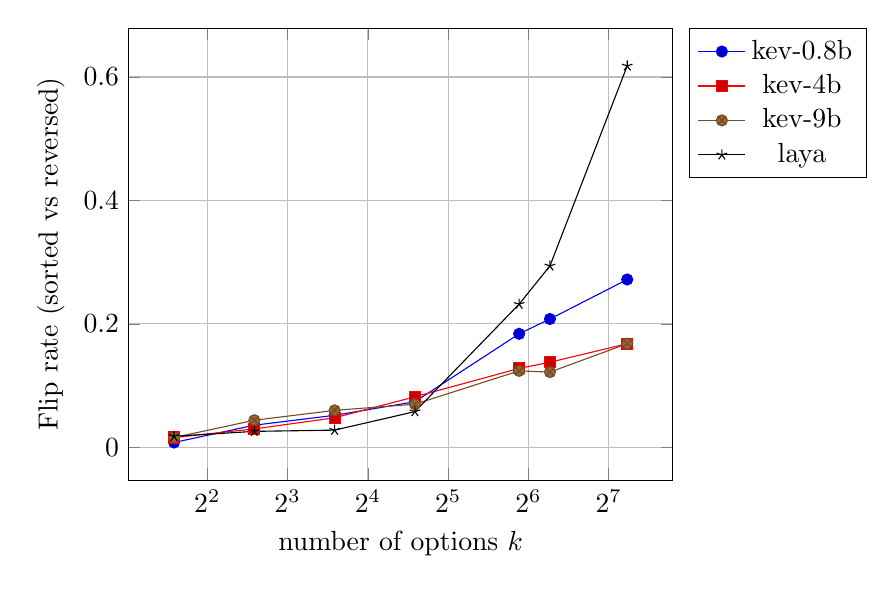
\begin{tikzpicture}
\begin{axis}[xlabel={number of options $k$}, ylabel={Flip rate (sorted vs reversed)}, xmode=log, log basis x=2, legend pos=outer north east, grid=major, width=0.7\linewidth]
\addplot coordinates { (3,0.0080) (6,0.0360) (12,0.0520) (24,0.0740) (59,0.1840) (77,0.2080) (150,0.2720) };
\addlegendentry{kev-0.8b}
\addplot coordinates { (3,0.0160) (6,0.0300) (12,0.0480) (24,0.0820) (59,0.1280) (77,0.1380) (150,0.1680) };
\addlegendentry{kev-4b}
\addplot coordinates { (3,0.0160) (6,0.0440) (12,0.0600) (24,0.0700) (59,0.1240) (77,0.1220) (150,0.1680) };
\addlegendentry{kev-9b}
\addplot coordinates { (3,0.0180) (6,0.0260) (12,0.0280) (24,0.0580) (59,0.2320) (77,0.2940) (150,0.6180) };
\addlegendentry{laya}
\end{axis}
\end{tikzpicture}

\caption{CLINC150: accuracy and flip rate vs number of options $k$.}
\end{figure}
\begin{figure}[h]\centering
% generated by cmd/plots, do not edit
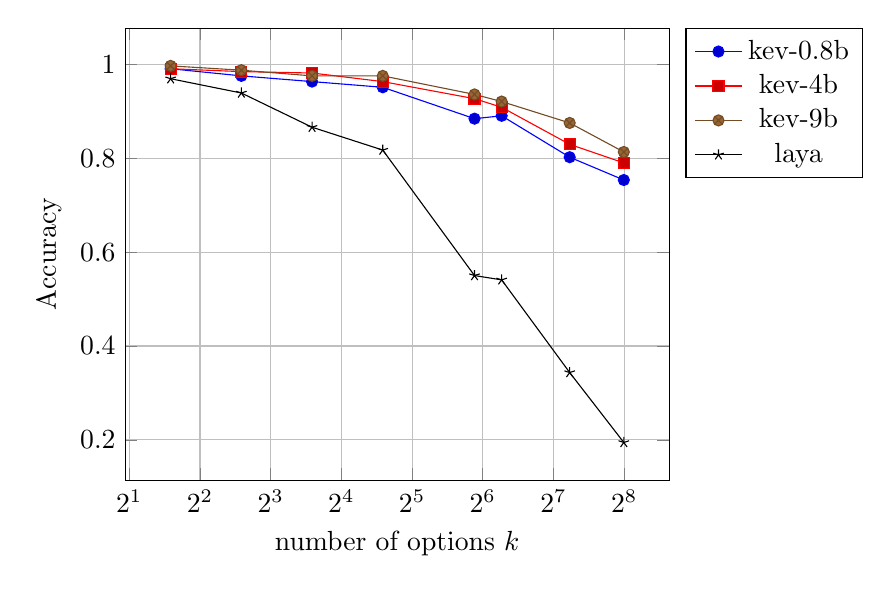
\begin{tikzpicture}
\begin{axis}[xlabel={number of options $k$}, ylabel={Accuracy}, xmode=log, log basis x=2, legend pos=outer north east, grid=major, width=0.7\linewidth]
\addplot coordinates { (3,0.9909) (6,0.9757) (12,0.9635) (24,0.9514) (59,0.8845) (77,0.8906) (150,0.8024) (255,0.7538) };
\addlegendentry{kev-0.8b}
\addplot coordinates { (3,0.9909) (6,0.9848) (12,0.9818) (24,0.9635) (59,0.9271) (77,0.9088) (150,0.8298) (255,0.7903) };
\addlegendentry{kev-4b}
\addplot coordinates { (3,0.9970) (6,0.9878) (12,0.9757) (24,0.9757) (59,0.9362) (77,0.9210) (150,0.8754) (255,0.8135) };
\addlegendentry{kev-9b}
\addplot coordinates { (3,0.9696) (6,0.9392) (12,0.8663) (24,0.8176) (59,0.5502) (77,0.5410) (150,0.3435) (255,0.1945) };
\addlegendentry{laya}
\end{axis}
\end{tikzpicture}

% generated by cmd/plots, do not edit
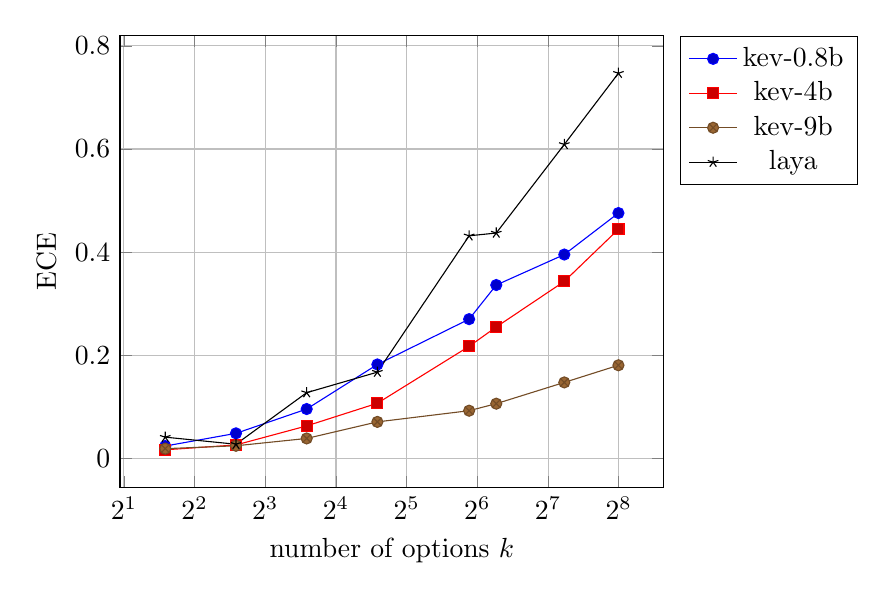
\begin{tikzpicture}
\begin{axis}[xlabel={number of options $k$}, ylabel={ECE}, xmode=log, log basis x=2, legend pos=outer north east, grid=major, width=0.7\linewidth]
\addplot coordinates { (3,0.0244) (6,0.0490) (12,0.0961) (24,0.1825) (59,0.2703) (77,0.3364) (150,0.3955) (255,0.4759) };
\addlegendentry{kev-0.8b}
\addplot coordinates { (3,0.0171) (6,0.0265) (12,0.0634) (24,0.1073) (59,0.2176) (77,0.2551) (150,0.3435) (255,0.4445) };
\addlegendentry{kev-4b}
\addplot coordinates { (3,0.0193) (6,0.0249) (12,0.0391) (24,0.0712) (59,0.0929) (77,0.1065) (150,0.1477) (255,0.1809) };
\addlegendentry{kev-9b}
\addplot coordinates { (3,0.0416) (6,0.0279) (12,0.1278) (24,0.1676) (59,0.4318) (77,0.4372) (150,0.6089) (255,0.7469) };
\addlegendentry{laya}
\end{axis}
\end{tikzpicture}

\caption{BFCL: accuracy and ECE vs $k$.}
\end{figure}
{\small% generated by cmd/eval-diagnose-k, do not edit
\begin{longtable}{llrrrrrr}
\toprule
Dataset & Model & $k$ & Acc & Acc (rev.) & ECE & Flip & p50 (ms) \\
\midrule
\endfirsthead
\toprule
Dataset & Model & $k$ & Acc & Acc (rev.) & ECE & Flip & p50 (ms) \\
\midrule
\endhead
banking77 & kev-0.8b & 3 & 0.986 & 0.988 & 0.025 & 0.002 & 51.6 \\
banking77 & kev-0.8b & 6 & 0.986 & 0.980 & 0.053 & 0.014 & 55.8 \\
banking77 & kev-0.8b & 12 & 0.966 & 0.970 & 0.075 & 0.018 & 65.6 \\
banking77 & kev-0.8b & 24 & 0.920 & 0.924 & 0.085 & 0.030 & 84.6 \\
banking77 & kev-0.8b & 59 & 0.882 & 0.870 & 0.145 & 0.058 & 151.5 \\
banking77 & kev-0.8b & 77 & 0.866 & 0.850 & 0.172 & 0.072 & 178.8 \\
banking77 & kev-4b & 3 & 0.990 & 0.988 & 0.020 & 0.010 & 230.9 \\
banking77 & kev-4b & 6 & 0.976 & 0.980 & 0.031 & 0.008 & 239.3 \\
banking77 & kev-4b & 12 & 0.966 & 0.962 & 0.071 & 0.014 & 271.0 \\
banking77 & kev-4b & 24 & 0.938 & 0.936 & 0.078 & 0.038 & 329.2 \\
banking77 & kev-4b & 59 & 0.894 & 0.894 & 0.114 & 0.050 & 468.1 \\
banking77 & kev-4b & 77 & 0.880 & 0.884 & 0.130 & 0.054 & 563.1 \\
banking77 & kev-9b & 3 & 0.988 & 0.990 & 0.018 & 0.010 & 377.4 \\
banking77 & kev-9b & 6 & 0.978 & 0.984 & 0.025 & 0.016 & 390.2 \\
banking77 & kev-9b & 12 & 0.964 & 0.966 & 0.034 & 0.020 & 436.8 \\
banking77 & kev-9b & 24 & 0.942 & 0.940 & 0.032 & 0.036 & 574.7 \\
banking77 & kev-9b & 59 & 0.892 & 0.900 & 0.034 & 0.052 & 770.1 \\
banking77 & kev-9b & 77 & 0.888 & 0.892 & 0.041 & 0.064 & 932.3 \\
banking77 & laya & 3 & 0.940 & 0.920 & 0.057 & 0.056 & 93.6 \\
banking77 & laya & 6 & 0.886 & 0.902 & 0.053 & 0.056 & 113.7 \\
banking77 & laya & 12 & 0.846 & 0.822 & 0.143 & 0.102 & 119.9 \\
banking77 & laya & 24 & 0.744 & 0.722 & 0.242 & 0.184 & 134.4 \\
banking77 & laya & 59 & 0.422 & 0.408 & 0.561 & 0.424 & 150.3 \\
banking77 & laya & 77 & 0.380 & 0.358 & 0.597 & 0.496 & 164.7 \\
bfcl & kev-0.8b & 3 & 0.991 & 0.997 & 0.024 & 0.006 & 66.8 \\
bfcl & kev-0.8b & 6 & 0.976 & 0.979 & 0.049 & 0.015 & 83.0 \\
bfcl & kev-0.8b & 12 & 0.964 & 0.954 & 0.096 & 0.036 & 122.8 \\
bfcl & kev-0.8b & 24 & 0.951 & 0.954 & 0.182 & 0.033 & 208.2 \\
bfcl & kev-0.8b & 59 & 0.884 & 0.869 & 0.270 & 0.085 & 247.8 \\
bfcl & kev-0.8b & 77 & 0.891 & 0.894 & 0.336 & 0.088 & 324.6 \\
bfcl & kev-0.8b & 150 & 0.802 & 0.802 & 0.396 & 0.173 & 1325.6 \\
bfcl & kev-0.8b & 255 & 0.754 & 0.739 & 0.476 & 0.243 & 1205.7 \\
bfcl & kev-4b & 3 & 0.991 & 0.997 & 0.017 & 0.006 & 268.1 \\
bfcl & kev-4b & 6 & 0.985 & 0.985 & 0.026 & 0.006 & 320.8 \\
bfcl & kev-4b & 12 & 0.982 & 0.973 & 0.063 & 0.021 & 406.0 \\
bfcl & kev-4b & 24 & 0.964 & 0.967 & 0.107 & 0.036 & 657.7 \\
bfcl & kev-4b & 59 & 0.927 & 0.921 & 0.218 & 0.061 & 713.4 \\
bfcl & kev-4b & 77 & 0.909 & 0.915 & 0.255 & 0.082 & 925.6 \\
bfcl & kev-4b & 150 & 0.830 & 0.851 & 0.343 & 0.140 & 3638.8 \\
bfcl & kev-4b & 255 & 0.790 & 0.805 & 0.444 & 0.195 & 3051.7 \\
bfcl & kev-9b & 3 & 0.997 & 0.994 & 0.019 & 0.003 & 467.2 \\
bfcl & kev-9b & 6 & 0.988 & 0.994 & 0.025 & 0.006 & 576.5 \\
bfcl & kev-9b & 12 & 0.976 & 0.979 & 0.039 & 0.015 & 696.8 \\
bfcl & kev-9b & 24 & 0.976 & 0.976 & 0.071 & 0.027 & 1042.0 \\
bfcl & kev-9b & 59 & 0.936 & 0.939 & 0.093 & 0.049 & 1155.1 \\
bfcl & kev-9b & 77 & 0.921 & 0.930 & 0.106 & 0.040 & 1462.7 \\
bfcl & kev-9b & 150 & 0.875 & 0.860 & 0.148 & 0.079 & 5266.0 \\
bfcl & kev-9b & 255 & 0.815 & 0.830 & 0.182 & 0.137 & 2325.1 \\
bfcl & laya & 3 & 0.970 & 0.985 & 0.042 & 0.030 & 19.8 \\
bfcl & laya & 6 & 0.939 & 0.945 & 0.028 & 0.043 & 29.5 \\
bfcl & laya & 12 & 0.866 & 0.903 & 0.128 & 0.125 & 34.7 \\
bfcl & laya & 24 & 0.818 & 0.799 & 0.168 & 0.167 & 34.4 \\
bfcl & laya & 59 & 0.550 & 0.578 & 0.432 & 0.307 & 41.3 \\
bfcl & laya & 77 & 0.541 & 0.547 & 0.437 & 0.343 & 54.5 \\
bfcl & laya & 150 & 0.343 & 0.398 & 0.609 & 0.678 & 111.8 \\
bfcl & laya & 255 & 0.195 & 0.243 & 0.747 & 0.866 & 86.7 \\
bfcl-nodesc & laya & 3 & 0.967 & 0.976 & 0.053 & 0.021 & 49.7 \\
bfcl-nodesc & laya & 6 & 0.924 & 0.942 & 0.027 & 0.040 & 52.8 \\
bfcl-nodesc & laya & 12 & 0.909 & 0.915 & 0.088 & 0.076 & 70.0 \\
bfcl-nodesc & laya & 24 & 0.866 & 0.860 & 0.125 & 0.100 & 95.3 \\
bfcl-nodesc & laya & 59 & 0.553 & 0.574 & 0.428 & 0.298 & 125.6 \\
bfcl-nodesc & laya & 77 & 0.541 & 0.544 & 0.437 & 0.334 & 152.2 \\
bfcl-nodesc & laya & 150 & 0.340 & 0.386 & 0.616 & 0.687 & 271.6 \\
bfcl-nodesc & laya & 255 & 0.195 & 0.252 & 0.752 & 0.872 & 206.6 \\
clinc150 & kev-0.8b & 3 & 0.968 & 0.972 & 0.032 & 0.008 & 56.7 \\
clinc150 & kev-0.8b & 6 & 0.910 & 0.920 & 0.038 & 0.036 & 52.4 \\
clinc150 & kev-0.8b & 12 & 0.876 & 0.870 & 0.048 & 0.052 & 58.6 \\
clinc150 & kev-0.8b & 24 & 0.816 & 0.812 & 0.073 & 0.074 & 71.0 \\
clinc150 & kev-0.8b & 59 & 0.768 & 0.740 & 0.150 & 0.184 & 112.5 \\
clinc150 & kev-0.8b & 77 & 0.732 & 0.686 & 0.160 & 0.208 & 136.2 \\
clinc150 & kev-0.8b & 150 & 0.654 & 0.606 & 0.197 & 0.272 & 232.2 \\
clinc150 & kev-4b & 3 & 0.982 & 0.984 & 0.043 & 0.016 & 221.2 \\
clinc150 & kev-4b & 6 & 0.950 & 0.950 & 0.061 & 0.030 & 228.4 \\
clinc150 & kev-4b & 12 & 0.944 & 0.934 & 0.116 & 0.048 & 245.7 \\
clinc150 & kev-4b & 24 & 0.886 & 0.890 & 0.147 & 0.082 & 277.7 \\
clinc150 & kev-4b & 59 & 0.860 & 0.836 & 0.237 & 0.128 & 383.0 \\
clinc150 & kev-4b & 77 & 0.838 & 0.804 & 0.262 & 0.138 & 433.8 \\
clinc150 & kev-4b & 150 & 0.774 & 0.752 & 0.302 & 0.168 & 743.4 \\
clinc150 & kev-9b & 3 & 0.970 & 0.972 & 0.039 & 0.016 & 383.4 \\
clinc150 & kev-9b & 6 & 0.958 & 0.956 & 0.052 & 0.044 & 396.2 \\
clinc150 & kev-9b & 12 & 0.936 & 0.948 & 0.073 & 0.060 & 416.2 \\
clinc150 & kev-9b & 24 & 0.910 & 0.924 & 0.096 & 0.070 & 491.2 \\
clinc150 & kev-9b & 59 & 0.880 & 0.862 & 0.150 & 0.124 & 670.8 \\
clinc150 & kev-9b & 77 & 0.854 & 0.844 & 0.154 & 0.122 & 732.6 \\
clinc150 & kev-9b & 150 & 0.792 & 0.798 & 0.175 & 0.168 & 1132.4 \\
clinc150 & laya & 3 & 0.982 & 0.988 & 0.046 & 0.018 & 14.4 \\
clinc150 & laya & 6 & 0.972 & 0.978 & 0.013 & 0.026 & 15.1 \\
clinc150 & laya & 12 & 0.962 & 0.974 & 0.034 & 0.028 & 17.7 \\
clinc150 & laya & 24 & 0.942 & 0.946 & 0.053 & 0.058 & 22.6 \\
clinc150 & laya & 59 & 0.790 & 0.754 & 0.193 & 0.232 & 36.5 \\
clinc150 & laya & 77 & 0.756 & 0.690 & 0.227 & 0.294 & 44.1 \\
clinc150 & laya & 150 & 0.532 & 0.490 & 0.448 & 0.618 & 93.2 \\
massive & kev-0.8b & 3 & 0.950 & 0.944 & 0.048 & 0.026 & 88.4 \\
massive & kev-0.8b & 6 & 0.896 & 0.898 & 0.077 & 0.062 & 55.2 \\
massive & kev-0.8b & 12 & 0.844 & 0.868 & 0.111 & 0.090 & 63.5 \\
massive & kev-0.8b & 24 & 0.728 & 0.766 & 0.104 & 0.184 & 81.7 \\
massive & kev-0.8b & 59 & 0.600 & 0.610 & 0.128 & 0.314 & 135.4 \\
massive & kev-4b & 3 & 0.964 & 0.962 & 0.043 & 0.018 & 226.9 \\
massive & kev-4b & 6 & 0.912 & 0.912 & 0.081 & 0.046 & 232.8 \\
massive & kev-4b & 12 & 0.880 & 0.876 & 0.141 & 0.082 & 252.0 \\
massive & kev-4b & 24 & 0.808 & 0.834 & 0.173 & 0.124 & 309.4 \\
massive & kev-4b & 59 & 0.692 & 0.754 & 0.216 & 0.240 & 416.7 \\
massive & kev-9b & 3 & 0.962 & 0.966 & 0.043 & 0.016 & 374.2 \\
massive & kev-9b & 6 & 0.924 & 0.902 & 0.066 & 0.058 & 379.5 \\
massive & kev-9b & 12 & 0.888 & 0.874 & 0.092 & 0.086 & 407.4 \\
massive & kev-9b & 24 & 0.832 & 0.834 & 0.120 & 0.124 & 514.0 \\
massive & kev-9b & 59 & 0.730 & 0.754 & 0.153 & 0.230 & 701.1 \\
massive & laya & 3 & 0.894 & 0.894 & 0.098 & 0.080 & 110.5 \\
massive & laya & 6 & 0.828 & 0.838 & 0.059 & 0.112 & 92.3 \\
massive & laya & 12 & 0.728 & 0.738 & 0.243 & 0.222 & 114.2 \\
massive & laya & 24 & 0.606 & 0.642 & 0.361 & 0.304 & 125.4 \\
massive & laya & 59 & 0.428 & 0.422 & 0.498 & 0.566 & 125.2 \\
\bottomrule
\end{longtable}
}
% TODO text:
% - Laya: best or equal up to k=24 (0.94-0.98) at 15-23 ms; collapses between
%   24 and 59 (192-token budget: 3 tokens per option at k=59, names truncated).
%   Identical numbers without descriptions (bfcl-nodesc) => budget, not descriptions.
% - Flip rate rises with k for all models: Laya 0.62 at k=150, 0.87 at k=255;
%   Kev-9B 0.17 at k=150.
% - ECE rises with k: confidence at large k is meaningless (Laya 0.45-0.75).

\section{Method: tournament querying}
% TODO: algorithm box. Shuffle, groups of G, one call per group, winner
% (tournament) or every option with p >= eps (adaptive) passes, repeat while
% > G candidates, final call. Chain: final p times product of round p.
% Permute: R shuffles, average. Cost: calls per decision.
\subsection{Conformal selection of $\varepsilon$}
% TODO: survival S(eps) = P(gold among finalists). Not monotone in eps (small
% eps => many rounds => more chances to drop gold; large eps => plain
% tournament). Hence split calibration in halves: A picks the largest eps with
% empirical miss rate <= alpha; B certifies (misses_B + 1)/(n_B + 1) <= alpha.
% One hypothesis tested on fresh data => valid without monotonicity.

\section{Results}
\subsection{Tournament vs single call}
{\small% generated by cmd/eval-tournament, do not edit
\begin{longtable}{llrrrrrrrrrrrr}
\toprule
 &  & \multicolumn{3}{c}{laya} & \multicolumn{3}{c}{kev-0.8b} & \multicolumn{3}{c}{kev-4b} & \multicolumn{3}{c}{kev-9b} \\
\cmidrule(lr){3-5}\cmidrule(lr){6-8}\cmidrule(lr){9-11}\cmidrule(lr){12-14}
Dataset & Method & Acc & ECE & Calls & Acc & ECE & Calls & Acc & ECE & Calls & Acc & ECE & Calls \\
\midrule
\endfirsthead
\toprule
 &  & \multicolumn{3}{c}{laya} & \multicolumn{3}{c}{kev-0.8b} & \multicolumn{3}{c}{kev-4b} & \multicolumn{3}{c}{kev-9b} \\
\cmidrule(lr){3-5}\cmidrule(lr){6-8}\cmidrule(lr){9-11}\cmidrule(lr){12-14}
Dataset & Method & Acc & ECE & Calls & Acc & ECE & Calls & Acc & ECE & Calls & Acc & ECE & Calls \\
\midrule
\endhead
clinc150 & single & 0.530 & 0.45 & 1.0 & 0.654 & 0.20 & 1.0 & 0.776 & 0.30 & 1.0 & 0.792 & 0.18 & 1.0 \\
clinc150 & permute-r4 & 0.596 & 0.08 & 4.0 & 0.672 & 0.25 & 4.0 & 0.782 & 0.33 & 4.0 & 0.826 & 0.26 & 4.0 \\
clinc150 & permute-r8 & 0.622 & 0.05 & 8.0 & 0.660 & 0.24 & 8.0 & 0.800 & 0.35 & 8.0 & 0.828 & 0.27 & 8.0 \\
clinc150 & tournament-g8 & 0.840 & 0.05 & 23.0 & 0.570 & 0.10 & 23.0 & 0.724 & 0.12 & 23.0 & 0.714 & 0.07 & 23.0 \\
clinc150 & tournament-g12 & 0.814 & 0.08 & 16.0 & 0.594 & 0.28 & 16.0 & 0.722 & 0.14 & 16.0 & 0.726 & 0.14 & 16.0 \\
clinc150 & tournament-g24 & 0.848 & 0.07 & 8.0 & 0.598 & 0.09 & 8.0 & 0.706 & 0.19 & 8.0 & 0.728 & 0.15 & 8.0 \\
clinc150 & adaptive-g12-eps0p05 & 0.830 & 0.02 & 16.0 & 0.580 & 0.14 & 20.3 & 0.684 & 0.26 & 20.6 & 0.684 & 0.20 & 20.2 \\
clinc150 & adaptive-g12-eps0p1 & 0.822 & 0.05 & 16.0 & 0.564 & 0.10 & 16.9 & 0.686 & 0.24 & 17.0 & 0.680 & 0.15 & 16.9 \\
clinc150 & chain-g12-eps0p1 & 0.828 & 0.06 & 16.0 & 0.594 & 0.06 & 16.9 & 0.754 & 0.10 & 17.0 & 0.764 & 0.06 & 16.9 \\
clinc150 & chain-g24-eps0p1 & 0.856 & 0.10 & 8.0 & 0.622 & 0.11 & 8.0 & 0.732 & 0.19 & 8.0 & 0.774 & 0.13 & 8.0 \\
\midrule
bfcl & single & 0.195 & 0.75 & 1.0 & 0.754 & 0.48 & 1.0 & 0.790 & 0.44 & 1.0 & 0.815 & 0.18 & 1.0 \\
bfcl & permute-r4 & 0.283 & 0.22 & 4.0 & 0.766 & 0.51 & 4.0 & 0.812 & 0.51 & 4.0 & 0.836 & 0.22 & 4.0 \\
bfcl & permute-r8 & 0.301 & 0.14 & 8.0 & 0.790 & 0.54 & 8.0 & 0.821 & 0.52 & 8.0 & 0.848 & 0.24 & 8.0 \\
bfcl & tournament-g8 & 0.590 & 0.15 & 37.0 & 0.769 & 0.12 & 37.0 & 0.793 & 0.07 & 37.0 & 0.818 & 0.04 & 37.0 \\
bfcl & tournament-g12 & 0.571 & 0.25 & 25.0 & 0.760 & 0.05 & 25.0 & 0.812 & 0.04 & 25.0 & 0.809 & 0.07 & 25.0 \\
bfcl & tournament-g24 & 0.544 & 0.42 & 12.0 & 0.769 & 0.24 & 12.0 & 0.830 & 0.17 & 12.0 & 0.842 & 0.10 & 12.0 \\
bfcl & adaptive-g12-eps0p05 & 0.584 & 0.18 & 26.0 & 0.751 & 0.22 & 39.8 & 0.802 & 0.15 & 39.2 & 0.833 & 0.09 & 45.3 \\
bfcl & adaptive-g12-eps0p1 & 0.602 & 0.17 & 25.9 & 0.769 & 0.21 & 28.5 & 0.812 & 0.14 & 28.6 & 0.839 & 0.11 & 28.0 \\
bfcl & chain-g12-eps0p1 & 0.602 & 0.20 & 25.9 & 0.760 & 0.06 & 28.5 & 0.818 & 0.05 & 28.6 & 0.830 & 0.04 & 28.0 \\
bfcl & chain-g24-eps0p1 & 0.565 & 0.40 & 12.0 & 0.769 & 0.15 & 12.3 & 0.818 & 0.11 & 12.1 & 0.842 & 0.07 & 12.0 \\
\midrule
bfcl-nodesc & single & 0.195 & 0.75 & 1.0 & -- & -- & -- & -- & -- & -- & -- & -- & -- \\
bfcl-nodesc & permute-r8 & 0.310 & 0.13 & 8.0 & -- & -- & -- & -- & -- & -- & -- & -- & -- \\
bfcl-nodesc & tournament-g8 & 0.629 & 0.13 & 37.0 & -- & -- & -- & -- & -- & -- & -- & -- & -- \\
bfcl-nodesc & tournament-g24 & 0.611 & 0.38 & 12.0 & -- & -- & -- & -- & -- & -- & -- & -- & -- \\
bfcl-nodesc & adaptive-g12-eps0p05 & 0.623 & 0.19 & 26.0 & -- & -- & -- & -- & -- & -- & -- & -- & -- \\
\midrule
massive & single & 0.426 & 0.50 & 1.0 & 0.600 & 0.13 & 1.0 & 0.692 & 0.22 & 1.0 & 0.730 & 0.15 & 1.0 \\
massive & permute-r4 & 0.414 & 0.23 & 4.0 & 0.634 & 0.16 & 4.0 & 0.760 & 0.28 & 4.0 & 0.728 & 0.20 & 4.0 \\
massive & permute-r8 & 0.440 & 0.16 & 8.0 & 0.636 & 0.17 & 8.0 & 0.762 & 0.28 & 8.0 & 0.732 & 0.21 & 8.0 \\
massive & tournament-g8 & 0.526 & 0.19 & 9.0 & 0.604 & 0.05 & 9.0 & 0.698 & 0.13 & 9.0 & 0.694 & 0.07 & 9.0 \\
massive & tournament-g12 & 0.540 & 0.08 & 6.0 & 0.588 & 0.06 & 6.0 & 0.680 & 0.09 & 6.0 & 0.682 & 0.05 & 6.0 \\
massive & tournament-g24 & 0.494 & 0.22 & 4.0 & 0.602 & 0.12 & 4.0 & 0.694 & 0.06 & 4.0 & 0.688 & 0.05 & 4.0 \\
massive & adaptive-g12-eps0p05 & 0.546 & 0.14 & 6.0 & 0.614 & 0.05 & 8.2 & 0.698 & 0.17 & 8.2 & 0.672 & 0.06 & 8.2 \\
massive & adaptive-g12-eps0p1 & 0.546 & 0.13 & 6.0 & 0.584 & 0.05 & 6.5 & 0.700 & 0.14 & 6.7 & 0.678 & 0.07 & 6.3 \\
massive & chain-g12-eps0p1 & 0.546 & 0.13 & 6.0 & 0.594 & 0.08 & 6.5 & 0.714 & 0.04 & 6.7 & 0.686 & 0.04 & 6.3 \\
massive & chain-g24-eps0p1 & 0.502 & 0.20 & 4.0 & 0.626 & 0.07 & 4.0 & 0.704 & 0.05 & 4.0 & 0.684 & 0.04 & 4.0 \\
\midrule
banking77 & single & 0.380 & 0.60 & 1.0 & 0.866 & 0.17 & 1.0 & 0.880 & 0.13 & 1.0 & 0.886 & 0.03 & 1.0 \\
banking77 & permute-r4 & 0.372 & 0.36 & 4.0 & 0.862 & 0.16 & 4.0 & 0.890 & 0.14 & 4.0 & 0.894 & 0.05 & 4.0 \\
banking77 & permute-r8 & 0.384 & 0.31 & 8.0 & 0.872 & 0.17 & 8.0 & 0.884 & 0.14 & 8.0 & 0.890 & 0.05 & 8.0 \\
banking77 & tournament-g8 & 0.626 & 0.21 & 13.0 & 0.850 & 0.07 & 13.0 & 0.856 & 0.07 & 13.0 & 0.868 & 0.07 & 13.0 \\
banking77 & tournament-g12 & 0.620 & 0.22 & 8.0 & 0.860 & 0.07 & 8.0 & 0.864 & 0.07 & 8.0 & 0.884 & 0.03 & 8.0 \\
banking77 & tournament-g24 & 0.610 & 0.16 & 5.0 & 0.856 & 0.03 & 5.0 & 0.876 & 0.04 & 5.0 & 0.878 & 0.02 & 5.0 \\
banking77 & adaptive-g12-eps0p05 & 0.624 & 0.29 & 8.4 & 0.858 & 0.08 & 11.9 & 0.876 & 0.09 & 10.6 & 0.884 & 0.03 & 10.6 \\
banking77 & adaptive-g12-eps0p1 & 0.634 & 0.25 & 8.2 & 0.850 & 0.04 & 9.9 & 0.876 & 0.05 & 9.8 & 0.878 & 0.03 & 9.7 \\
banking77 & chain-g12-eps0p1 & 0.636 & 0.26 & 8.2 & 0.866 & 0.04 & 9.9 & 0.886 & 0.03 & 9.8 & 0.882 & 0.06 & 9.7 \\
banking77 & chain-g24-eps0p1 & 0.610 & 0.24 & 5.0 & 0.862 & 0.03 & 5.0 & 0.880 & 0.04 & 5.0 & 0.894 & 0.04 & 5.0 \\
\bottomrule
\end{longtable}
}
\begin{figure}[h]\centering
% generated by cmd/plots, do not edit
\begin{tikzpicture}
\begin{axis}[xlabel={latency p50 (ms)}, ylabel={Accuracy}, xmode=log, legend pos=south west, legend style={font=\scriptsize}, label style={font=\small}, tick label style={font=\scriptsize}, grid=major, width=\plotwidth, height=0.72\plotwidth, nodes near coords, every node near coord/.append style={font=\tiny, anchor=west, rotate=20}, point meta=explicit symbolic]
\addplot+[only marks, mark=*] coordinates { (1193.233,0.5720) [adaptive-g12-eps0p05] (981.53,0.5660) [adaptive-g12-eps0p1] (955.773,0.5820) [chain-g12-eps2] (576.533,0.6140) [chain-g24-eps2] (954.674,0.6740) [permute-r4] (1904.789,0.6600) [permute-r8] (321.499,0.6540) [single] (916.475,0.5980) [tournament-g12] (540.961,0.5960) [tournament-g24] (1241.579,0.5600) [tournament-g8] };
\addlegendentry{kev-0.8b}
\addplot+[only marks, mark=*] coordinates { (5232.067,0.6780) [adaptive-g12-eps0p05] (4256.1,0.6920) [adaptive-g12-eps0p1] (4102.377,0.6880) [chain-g12-eps2] (2273.233,0.7300) [chain-g24-eps2] (2875.395,0.7820) [permute-r4] (5753.133,0.8000) [permute-r8] (718.646,0.7740) [single] (3964.731,0.7200) [tournament-g12] (2184.414,0.7060) [tournament-g24] (5446.268,0.7240) [tournament-g8] };
\addlegendentry{kev-4b}
\addplot+[only marks, mark=*] coordinates { (8774.469,0.6880) [adaptive-g12-eps0p05] (7165.579,0.6880) [adaptive-g12-eps0p1] (6881.559,0.7100) [chain-g12-eps2] (3899.464,0.7620) [chain-g24-eps2] (4250.742,0.8260) [permute-r4] (8512.169,0.8280) [permute-r8] (1064.642,0.7920) [single] (6680.363,0.7260) [tournament-g12] (3799.424,0.7280) [tournament-g24] (9352.723,0.7140) [tournament-g8] };
\addlegendentry{kev-9b}
\addplot+[only marks, mark=*] coordinates { (296.135,0.8280) [adaptive-g12-eps0p05] (278.859,0.8240) [adaptive-g12-eps0p1] (378.809,0.5980) [permute-r4] (711.96,0.6220) [permute-r8] (92.359,0.5320) [single] (323.188,0.8160) [tournament-g12] (218.994,0.8420) [tournament-g24] (397.745,0.8380) [tournament-g8] };
\addlegendentry{laya}
\end{axis}
\end{tikzpicture}

\caption{CLINC150, $k=150$: accuracy vs latency per method and model.}
\end{figure}
% TODO text:
% - Laya CLINC150: 0.532 -> 0.842 (tournament G=24, 8 calls, 219 ms), ECE
%   0.447 -> 0.068. Beats Kev-9B single (0.792, 1.1 s) and Qwen2.5-7B (0.792, 0.9 s).
% - Kev: tournament lowers accuracy (Kev-9B 0.792 -> 0.73), chain recovers
%   part (0.762 at G=24), permute helps (+3-4 pp, 0.828). Mechanism: per-round
%   errors compound; final = hard negatives.
% - Laya BFCL: 0.195 -> 0.63 (tournament G=8, no descriptions); still below
%   Kev (0.82-0.85). Explained by per-round accuracy 0.87-0.91 at k=8-12 and
%   3 rounds: 0.9^3 ~ 0.73.
\subsection{Survival guarantee}
{\small% generated by cmd/eval-calibrate, do not edit
\begin{tabular}{lllrrlrrr}
\toprule
Dataset & Model & Method & $\alpha$ & $\varepsilon$ & Certified & Test survival & Acc & Calls \\
\midrule
clinc150 & kev-0.8b & adaptive-g12 & 0.10 & 0.050 & no & 0.916 & 0.576 & 20.3 \\
clinc150 & kev-0.8b & adaptive-g12 & 0.20 & 0.100 & yes & 0.892 & 0.558 & 16.9 \\
clinc150 & kev-4b & adaptive-g12 & 0.05 & 0.100 & no & 0.940 & 0.688 & 17.0 \\
clinc150 & kev-4b & adaptive-g12 & 0.10 & 0.100 & yes & 0.940 & 0.688 & 17.0 \\
clinc150 & kev-4b & adaptive-g12 & 0.20 & 0.200 & yes & 0.844 & 0.722 & 16.0 \\
clinc150 & kev-9b & adaptive-g12 & 0.05 & 0.050 & no & 0.000 & 0.000 & 0.0 \\
clinc150 & kev-9b & adaptive-g12 & 0.10 & 0.100 & yes & 0.000 & 0.000 & 0.0 \\
clinc150 & kev-9b & adaptive-g12 & 0.20 & 0.300 & no & 0.000 & 0.000 & 0.0 \\
clinc150 & laya & adaptive-g12 & 0.10 & 0.300 & no & 0.854 & 0.810 & 16.0 \\
clinc150 & laya & adaptive-g12 & 0.20 & 0.500 & yes & 0.860 & 0.816 & 16.0 \\
\bottomrule
\end{tabular}
}
\begin{figure}[h]\centering
% generated by cmd/plots, do not edit
\begin{tikzpicture}
\begin{axis}[xlabel={calls per decision}, ylabel={Survival (test)}, xmode=log, legend pos=south west, legend style={font=\scriptsize}, label style={font=\small}, tick label style={font=\scriptsize}, grid=major, width=\plotwidth, height=0.72\plotwidth]
\addplot coordinates { (25,0.8784) (25.033434650455927,0.9301) (25.5531914893617,0.9422) (27.98480243161094,0.9726) (45.389057750759875,0.9787) (97.5775075987842,0.9848) (142.40425531914894,0.9757) };
\addlegendentry{adaptive-g12}
\addplot coordinates { (12,0.9878) (12,0.9787) (12,0.9757) (12,0.9726) (14.100303951367781,0.9726) (23.27659574468085,0.9909) (36.73252279635258,0.9909) };
\addlegendentry{adaptive-g24}
\addplot coordinates { (7,0.9848) (7,0.9757) (7,0.9635) (7,0.9635) (7,0.9483) (7.966565349544073,0.9818) (10.848024316109422,0.9939) };
\addlegendentry{adaptive-g48}
\end{axis}
\end{tikzpicture}

% generated by cmd/plots, do not edit
\begin{tikzpicture}
\begin{axis}[xlabel={calls per decision}, ylabel={Survival (test)}, xmode=log, legend pos=south west, legend style={font=\scriptsize}, label style={font=\small}, tick label style={font=\scriptsize}, grid=major, width=\plotwidth, height=0.72\plotwidth]
\addplot coordinates { (16,0.8700) (16,0.8540) (16,0.8600) (16.002,0.8960) (16.022,0.9040) (16.102,0.9120) (16.198,0.9060) (16.292,0.9320) (16.556,0.9240) };
\addlegendentry{adaptive-g12}
\addplot coordinates { (8,0.9620) (8,0.9620) (8,0.9600) (8,0.9580) (8,0.9580) (8,0.9560) (8,0.9540) };
\addlegendentry{adaptive-g24}
\addplot coordinates { (5,0.8280) (5,0.8260) (5,0.8160) (5,0.8160) (5,0.8140) (5,0.8060) (5,0.8040) };
\addlegendentry{adaptive-g48}
\end{axis}
\end{tikzpicture}

\caption{Test survival vs calls per decision for $G\in\{12,24,48\}$.}
\end{figure}
% TODO text: 45 certified (model, dataset, G, alpha) picks, 44 hold on test
% (miss: Kev-4B BFCL G=48 alpha=0.05, 0.945). Larger G = fewer rounds = higher
% survival and fewer calls; at G=24/48 eps=0.5 (plain tournament) usually
% suffices; small eps only for tight alpha and small G. Laya BFCL cannot be
% certified below alpha=0.2.
\subsection{Transfer of $\varepsilon$ between tasks}
{\small% generated by cmd/eval-transfer, do not edit
\begin{longtable}{llrllrrrl}
\toprule
Model & $G$ & $\alpha$ & Source & Target & $\varepsilon$ & Source surv. & Target surv. & Holds \\
\midrule
\endfirsthead
\toprule
Model & $G$ & $\alpha$ & Source & Target & $\varepsilon$ & Source surv. & Target surv. & Holds \\
\midrule
\endhead
kev-0.8b & 12 & 0.10 & banking77 & bfcl & 0.500 & 0.962 & 0.854 & no \\
kev-0.8b & 12 & 0.10 & banking77 & clinc150 & 0.500 & 0.962 & 0.644 & no \\
kev-0.8b & 12 & 0.10 & banking77 & massive & 0.500 & 0.962 & 0.838 & no \\
kev-0.8b & 12 & 0.20 & banking77 & massive & 0.500 & 0.962 & 0.838 & yes \\
kev-0.8b & 12 & 0.20 & banking77 & clinc150 & 0.500 & 0.962 & 0.644 & no \\
kev-0.8b & 12 & 0.20 & banking77 & bfcl & 0.500 & 0.962 & 0.854 & yes \\
kev-4b & 12 & 0.10 & banking77 & bfcl & 0.500 & 0.968 & 0.894 & no \\
kev-4b & 12 & 0.10 & banking77 & clinc150 & 0.500 & 0.968 & 0.736 & no \\
kev-4b & 12 & 0.10 & banking77 & massive & 0.500 & 0.968 & 0.874 & no \\
kev-4b & 12 & 0.20 & banking77 & bfcl & 0.500 & 0.968 & 0.894 & yes \\
kev-4b & 12 & 0.20 & banking77 & clinc150 & 0.500 & 0.968 & 0.736 & no \\
kev-4b & 12 & 0.20 & banking77 & massive & 0.500 & 0.968 & 0.874 & yes \\
kev-9b & 12 & 0.10 & banking77 & bfcl & 0.500 & 0.964 & 0.878 & no \\
kev-9b & 12 & 0.10 & banking77 & clinc150 & 0.500 & 0.964 & 0.756 & no \\
kev-9b & 12 & 0.10 & banking77 & massive & 0.500 & 0.964 & 0.892 & no \\
kev-9b & 12 & 0.20 & banking77 & bfcl & 0.500 & 0.964 & 0.878 & yes \\
kev-9b & 12 & 0.20 & banking77 & clinc150 & 0.500 & 0.964 & 0.756 & no \\
kev-9b & 12 & 0.20 & banking77 & massive & 0.500 & 0.964 & 0.892 & yes \\
laya & 12 & 0.20 & banking77 & bfcl & 0.500 & 0.846 & 0.650 & no \\
laya & 12 & 0.20 & banking77 & clinc150 & 0.500 & 0.846 & 0.860 & yes \\
laya & 12 & 0.20 & banking77 & massive & 0.500 & 0.846 & 0.730 & no \\
kev-0.8b & 12 & 0.05 & bfcl & banking77 & 0.100 & 0.960 & 0.962 & yes \\
kev-0.8b & 12 & 0.05 & bfcl & clinc150 & 0.100 & 0.960 & 0.892 & no \\
kev-0.8b & 12 & 0.05 & bfcl & massive & 0.100 & 0.960 & 0.916 & no \\
kev-0.8b & 12 & 0.10 & bfcl & banking77 & 0.200 & 0.939 & 0.982 & yes \\
kev-0.8b & 12 & 0.10 & bfcl & clinc150 & 0.200 & 0.939 & 0.748 & no \\
kev-0.8b & 12 & 0.10 & bfcl & massive & 0.200 & 0.939 & 0.914 & yes \\
kev-0.8b & 12 & 0.20 & bfcl & massive & 0.300 & 0.875 & 0.878 & yes \\
kev-0.8b & 12 & 0.20 & bfcl & clinc150 & 0.300 & 0.875 & 0.688 & no \\
kev-0.8b & 12 & 0.20 & bfcl & banking77 & 0.300 & 0.875 & 0.968 & yes \\
kev-0.8b & 24 & 0.05 & bfcl & clinc150 & 0.200 & 0.973 & 0.902 & no \\
kev-0.8b & 24 & 0.10 & bfcl & clinc150 & 0.500 & 0.957 & 0.816 & no \\
kev-0.8b & 24 & 0.20 & bfcl & clinc150 & 0.500 & 0.957 & 0.816 & yes \\
kev-0.8b & 48 & 0.05 & bfcl & clinc150 & 0.100 & 0.973 & 0.884 & no \\
kev-0.8b & 48 & 0.10 & bfcl & clinc150 & 0.300 & 0.954 & 0.794 & no \\
kev-0.8b & 48 & 0.20 & bfcl & clinc150 & 0.500 & 0.933 & 0.772 & no \\
kev-4b & 12 & 0.05 & bfcl & banking77 & 0.100 & 0.973 & 0.968 & yes \\
kev-4b & 12 & 0.05 & bfcl & clinc150 & 0.100 & 0.973 & 0.940 & no \\
kev-4b & 12 & 0.05 & bfcl & massive & 0.100 & 0.973 & 0.948 & no \\
kev-4b & 12 & 0.10 & bfcl & banking77 & 0.300 & 0.909 & 0.978 & yes \\
kev-4b & 12 & 0.10 & bfcl & clinc150 & 0.300 & 0.909 & 0.768 & no \\
kev-4b & 12 & 0.10 & bfcl & massive & 0.300 & 0.909 & 0.916 & yes \\
kev-4b & 12 & 0.20 & bfcl & banking77 & 0.500 & 0.894 & 0.968 & yes \\
kev-4b & 12 & 0.20 & bfcl & clinc150 & 0.500 & 0.894 & 0.736 & no \\
kev-4b & 12 & 0.20 & bfcl & massive & 0.500 & 0.894 & 0.874 & yes \\
kev-4b & 24 & 0.05 & bfcl & clinc150 & 0.500 & 0.964 & 0.910 & no \\
kev-4b & 24 & 0.10 & bfcl & clinc150 & 0.500 & 0.964 & 0.910 & yes \\
kev-4b & 24 & 0.20 & bfcl & clinc150 & 0.500 & 0.964 & 0.910 & yes \\
kev-4b & 48 & 0.05 & bfcl & clinc150 & 0.300 & 0.945 & 0.870 & no \\
kev-4b & 48 & 0.10 & bfcl & clinc150 & 0.500 & 0.936 & 0.862 & no \\
kev-4b & 48 & 0.20 & bfcl & clinc150 & 0.500 & 0.936 & 0.862 & yes \\
kev-9b & 12 & 0.05 & bfcl & clinc150 & 0.100 & 0.973 & 0.940 & no \\
kev-9b & 12 & 0.05 & bfcl & banking77 & 0.100 & 0.973 & 0.956 & yes \\
kev-9b & 12 & 0.05 & bfcl & massive & 0.100 & 0.973 & 0.948 & no \\
kev-9b & 12 & 0.10 & bfcl & banking77 & 0.300 & 0.930 & 0.972 & yes \\
kev-9b & 12 & 0.10 & bfcl & clinc150 & 0.300 & 0.930 & 0.794 & no \\
kev-9b & 12 & 0.10 & bfcl & massive & 0.300 & 0.930 & 0.912 & yes \\
kev-9b & 12 & 0.20 & bfcl & clinc150 & 0.500 & 0.878 & 0.756 & no \\
kev-9b & 12 & 0.20 & bfcl & banking77 & 0.500 & 0.878 & 0.964 & yes \\
kev-9b & 12 & 0.20 & bfcl & massive & 0.500 & 0.878 & 0.892 & yes \\
kev-9b & 24 & 0.05 & bfcl & clinc150 & 0.500 & 0.973 & 0.920 & no \\
kev-9b & 24 & 0.10 & bfcl & clinc150 & 0.500 & 0.973 & 0.920 & yes \\
kev-9b & 24 & 0.20 & bfcl & clinc150 & 0.500 & 0.973 & 0.920 & yes \\
kev-9b & 48 & 0.05 & bfcl & clinc150 & 0.200 & 0.964 & 0.906 & no \\
kev-9b & 48 & 0.10 & bfcl & clinc150 & 0.500 & 0.948 & 0.886 & no \\
kev-9b & 48 & 0.20 & bfcl & clinc150 & 0.500 & 0.948 & 0.886 & yes \\
laya & 24 & 0.20 & bfcl & clinc150 & 0.500 & 0.824 & 0.954 & yes \\
kev-0.8b & 12 & 0.20 & clinc150 & banking77 & 0.100 & 0.892 & 0.962 & yes \\
kev-0.8b & 12 & 0.20 & clinc150 & bfcl & 0.100 & 0.892 & 0.960 & yes \\
kev-0.8b & 12 & 0.20 & clinc150 & massive & 0.100 & 0.892 & 0.916 & yes \\
kev-0.8b & 24 & 0.10 & clinc150 & bfcl & 0.100 & 0.938 & 0.973 & yes \\
kev-0.8b & 24 & 0.20 & clinc150 & bfcl & 0.500 & 0.816 & 0.957 & yes \\
kev-0.8b & 48 & 0.05 & clinc150 & bfcl & 0.010 & 0.974 & 0.994 & yes \\
kev-0.8b & 48 & 0.10 & clinc150 & bfcl & 0.050 & 0.934 & 0.988 & yes \\
kev-0.8b & 48 & 0.20 & clinc150 & bfcl & 0.200 & 0.834 & 0.960 & yes \\
kev-4b & 12 & 0.10 & clinc150 & massive & 0.100 & 0.940 & 0.948 & yes \\
kev-4b & 12 & 0.10 & clinc150 & bfcl & 0.100 & 0.940 & 0.973 & yes \\
kev-4b & 12 & 0.10 & clinc150 & banking77 & 0.100 & 0.940 & 0.968 & yes \\
kev-4b & 12 & 0.20 & clinc150 & bfcl & 0.200 & 0.844 & 0.957 & yes \\
kev-4b & 12 & 0.20 & clinc150 & banking77 & 0.200 & 0.844 & 0.984 & yes \\
kev-4b & 12 & 0.20 & clinc150 & massive & 0.200 & 0.844 & 0.946 & yes \\
kev-4b & 24 & 0.10 & clinc150 & bfcl & 0.500 & 0.910 & 0.964 & yes \\
kev-4b & 24 & 0.20 & clinc150 & bfcl & 0.500 & 0.910 & 0.964 & yes \\
kev-4b & 48 & 0.20 & clinc150 & bfcl & 0.500 & 0.862 & 0.936 & yes \\
kev-9b & 12 & 0.10 & clinc150 & banking77 & 0.100 & 0.940 & 0.956 & yes \\
kev-9b & 12 & 0.10 & clinc150 & bfcl & 0.100 & 0.940 & 0.973 & yes \\
kev-9b & 12 & 0.10 & clinc150 & massive & 0.100 & 0.940 & 0.948 & yes \\
kev-9b & 24 & 0.20 & clinc150 & bfcl & 0.500 & 0.920 & 0.973 & yes \\
kev-9b & 48 & 0.20 & clinc150 & bfcl & 0.500 & 0.886 & 0.948 & yes \\
laya & 12 & 0.20 & clinc150 & banking77 & 0.500 & 0.860 & 0.846 & yes \\
laya & 12 & 0.20 & clinc150 & bfcl & 0.500 & 0.860 & 0.650 & no \\
laya & 12 & 0.20 & clinc150 & massive & 0.500 & 0.860 & 0.730 & no \\
laya & 24 & 0.10 & clinc150 & bfcl & 0.500 & 0.954 & 0.824 & no \\
laya & 24 & 0.20 & clinc150 & bfcl & 0.500 & 0.954 & 0.824 & yes \\
laya & 48 & 0.20 & clinc150 & bfcl & 0.500 & 0.804 & 0.647 & no \\
kev-0.8b & 12 & 0.05 & massive & clinc150 & 0.050 & 0.928 & 0.916 & no \\
kev-0.8b & 12 & 0.05 & massive & bfcl & 0.050 & 0.928 & 0.973 & yes \\
kev-0.8b & 12 & 0.05 & massive & banking77 & 0.050 & 0.928 & 0.980 & yes \\
kev-0.8b & 12 & 0.10 & massive & bfcl & 0.200 & 0.914 & 0.939 & yes \\
kev-0.8b & 12 & 0.10 & massive & clinc150 & 0.200 & 0.914 & 0.748 & no \\
kev-0.8b & 12 & 0.10 & massive & banking77 & 0.200 & 0.914 & 0.982 & yes \\
kev-0.8b & 12 & 0.20 & massive & banking77 & 0.500 & 0.838 & 0.962 & yes \\
kev-0.8b & 12 & 0.20 & massive & bfcl & 0.500 & 0.838 & 0.854 & yes \\
kev-0.8b & 12 & 0.20 & massive & clinc150 & 0.500 & 0.838 & 0.644 & no \\
kev-4b & 12 & 0.10 & massive & bfcl & 0.300 & 0.916 & 0.909 & yes \\
kev-4b & 12 & 0.10 & massive & banking77 & 0.300 & 0.916 & 0.978 & yes \\
kev-4b & 12 & 0.10 & massive & clinc150 & 0.300 & 0.916 & 0.768 & no \\
kev-4b & 12 & 0.20 & massive & bfcl & 0.500 & 0.874 & 0.894 & yes \\
kev-4b & 12 & 0.20 & massive & clinc150 & 0.500 & 0.874 & 0.736 & no \\
kev-4b & 12 & 0.20 & massive & banking77 & 0.500 & 0.874 & 0.968 & yes \\
kev-9b & 12 & 0.10 & massive & banking77 & 0.300 & 0.912 & 0.972 & yes \\
kev-9b & 12 & 0.10 & massive & bfcl & 0.300 & 0.912 & 0.930 & yes \\
kev-9b & 12 & 0.10 & massive & clinc150 & 0.300 & 0.912 & 0.794 & no \\
kev-9b & 12 & 0.20 & massive & bfcl & 0.500 & 0.892 & 0.878 & yes \\
kev-9b & 12 & 0.20 & massive & banking77 & 0.500 & 0.892 & 0.964 & yes \\
kev-9b & 12 & 0.20 & massive & clinc150 & 0.500 & 0.892 & 0.756 & no \\
\bottomrule
\end{longtable}
}
% TODO text: 23/46 certified eps hold on the other dataset; towards the easier
% task (BFCL) yes, towards CLINC150 no. eps must be calibrated per task
% (a few hundred labelled examples, minutes).
\subsection{LLM reference}
% generated by cmd/eval-llm, do not edit
\begin{tabular}{llrrrr}
\toprule
Dataset & Model & $k$ & Acc & Unparsed & p50 (ms) \\
\midrule
bfcl & qwen-7b & 12 & 0.979 & 2 & 515 \\
bfcl & qwen-7b & 255 & 0.733 & 4 & 7591 \\
clinc150 & qwen-7b & 12 & 0.980 & 0 & 172 \\
clinc150 & qwen-7b & 150 & 0.792 & 1 & 939 \\
\bottomrule
\end{tabular}

% TODO text: Qwen2.5-7B with the option list in the prompt: 0.792 at k=150
% (939 ms), 0.733 at k=255 (7.6 s). Laya + tournament is more accurate and
% 4x faster on CLINC150; Kev-9B single is more accurate on BFCL.

\section{Discussion}
% TODO: when to use what. Encoder with token budget: tournament, G as large
% as per-round accuracy allows. Decoder pointer model: permutation averaging.
% Rule: accuracy(tournament) ~ prod of per-round accuracies, predicts both.
% Limitations: two datasets in the tournament part, GGUF port vs PyTorch,
% latencies measured on shared GPU except cost tables, one seed.

\section{Conclusion}
% TODO

\bibliographystyle{plainnat}
\bibliography{refs}
\end{document}
